\chapter{File Formats}
\label{cha:formats}

\section{PyLith Mesh ASCII Files}
\label{sec:MeshIOAscii}

PyLith mesh ASCII files allow quick specification of the mesh information
for very small, simple meshes that are most easily written by hand.
We do not recommend using this format for anything other than these
very small, simple meshes.

\noindent \begin{center}
\begin{figure}[H]
\noindent \begin{centering}
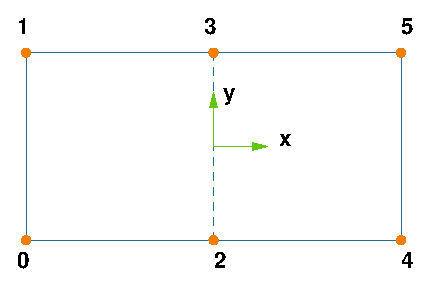
\includegraphics{fileformats/figs/meshquad4}
\par\end{centering}

\caption{Diagram of mesh specified in Figure \vref{fig:meshioascii:format}.\label{fig:meshioascii:diagram}}
\end{figure}

\par\end{center}
\begin{lyxcode}
//~This~mesh~file~defines~a~finite-element~mesh~composed~of~two

//~square~cells~of~edge~length~2.



//~Comments~can~appear~almost~anywhere~in~these~files~and~are

//~delimited~with~two~slashes~(//)~just~like~in~C++.~All~text~and~

//~whitespace~after~the~delimiter~on~a~given~line~is~ignored.

mesh~=~\{~//~begin~specification~of~the~mesh

~~dimension~=~2~//~spatial~dimension~of~the~mesh



~~//~Begin~vertex~and~cell~labels~with~0.~This~is~the~default~so~

~~//~this~next~line~is~optional

~~use-index-zero~=~true



~~vertices~=~\{~//~vertices~or~nodes~of~the~finite-element~cells

~~~~dimension~=~2~//~spatial~dimension~of~the~vertex~coordinates

~~~~count~=~6~//~number~of~vertices~in~the~mesh

~~~~coordinates~=~\{~//~list~of~vertex~index~and~coordinates

~~~~~~//~the~coordinates~must~coincide~with~the~coordinate~

~~~~~~//~system~specified~in~the~Mesh~object

~

~~~~~~//~exactly~one~vertex~must~appear~on~each~line

~~~~~~//~(excluding~whitespace)

~~~~~~0~~~~-2.0~~-1.0

~~~~~~1~~~~-2.0~~+1.0

~~~~~~2~~~~~0.0~~-1.0

~~~~~~3~~~~~0.0~~+1.0

~~~~~~4~~~~+2.0~~-1.0

~~~~~~5~~~~+2.0~~+1.0

~~~~\}~//~end~of~coordinates~list

~~\}~//~end~of~vertices

~

~~cells~=~\{~//~finite-element~cells

~~~~count~=~2~//~number~of~cells~in~the~mesh

~~~~num-corners~=~4~//~number~of~vertices~defining~the~cell

~~~~simplices~=~\{~//~list~of~vertices~in~each~cell

~~~~~~//~see~Section~4.2~for~diagrams~giving~the~order~for~each~

~~~~~~//~type~of~cell~supported~in~PyLith

~

~~~~~~//~index~of~cell~precedes~the~list~of~vertices~for~the~cell~



~~~~~~//~exactly~one~cell~must~appear~on~each~line

~~~~~~//~(excluding~whitespace)

~~~~~~0~~~~0~~2~~3~~1

~~~~~~1~~~~4~~5~~3~~2

~~~~\}~//~end~of~simplices~list

~

~~~~material-ids~=~\{~//~associated~each~cell~with~a~material~model

~~~~~~//~the~material~id~is~specified~using~the~index~of~the~cell~

~~~~~~//~and~then~the~corresponding~material~id

~~~~~~0~~~0~//~cell~0~has~a~material~id~of~0

~~~~~~1~~~2~//~cell~1~has~a~material~id~of~2

~~~~\}~//~end~of~material-ids~list

~~\}~//~end~of~cells

~

~~//~This~next~section~lists~groups~of~vertices~that~can~be~used

~~//~in~applying~boundary~conditions~to~portions~of~the~domain

~~group~=~\{~//~start~of~a~group

~~~~//~the~name~can~have~whitespace,~so~no~comments~are~allowed

~~~~//~after~the~name

~~~~name~=~face~+y

~

~~~~//~Either~groups~of~vertices~or~groups~of~cells~can~be~~~~~

~~~~//~specified,~but~currently~PyLith~only~makes~use~of~groups~

~~~~//~of~vertices

~~~~type~=~vertices~//~'vertices'~or~'cells'

~~~~count~=~2~//~number~of~vertices~in~the~group

~~~~indices~=~\{~//~list~of~vertex~indices~in~the~group

~~~~~~//~multiple~vertices~may~appear~on~a~line

~~~~~~0~~4~//~this~group~contains~vertices~0~and~4

~~~~\}~//~end~of~list~of~vertices

~~\}~//~end~of~group

~~//~additional~groups~can~be~listed~here
\end{lyxcode}
\begin{figure}[H]
\caption{Format of \texttt{PyLith} mesh ASCII files.\label{fig:meshioascii:format}}
\end{figure}



\section{SimpleDB Spatial Database Files}
\label{sec:spatialdata:SimpleIOAscii}

SimpleDB spatial database files contain a header describing the set
of points and then the data with each line listing the coordinates
of a point followed by the values of the fields for that point. 
\begin{lyxcode}
//~This~spatial~database~specifies~the~distribution~of~slip~on~the

//~fault~surface.~In~this~case~we~prescribe~a~piecewise~linear,~

//~depth~dependent~distribution~of~slip.~The~slip~is~2.0~m~

//~right-lateral~with~0.25~m~of~reverse~slip~at~the~surface~with

//~a~linear~taper~from~2.0~m~to~0.0~m~from~-2~km~to~-4~km.

~

//~Comments~can~appear~almost~anywhere~in~these~files~and~are

//~delimited~with~two~slashes~(//)~just~like~in~C++.~All~text~and~

//~whitespace~after~the~delimiter~on~a~given~line~is~ignored.

~

//~The~next~line~is~the~magic~header~for~spatial~database~files~

//~in~ASCII~format.

\#SPATIAL.ascii~1

SimpleDB~\{~//~start~specifying~the~database~parameters

~~num-values~=~3~//~number~of~values~in~the~database

~

~~//~Specify~the~names~and~the~order~of~the~values~as~they~appear~

~~//~in~the~data.~The~names~of~the~values~must~correspond~to~the~

~~//~names~PyLith~requests~in~querying~the~database.

~~value-names~=~~left-lateral-slip~~reverse-slip~~fault-opening

~

~~//~Specify~the~units~of~the~values~in~Python~syntax~(e.g.,~kg/m{*}{*}3).

~~value-units~=~~m~~m~~m



~~num-locs~=~3~//~Number~of~locations~where~values~are~given

~~data-dim~=~1~//~Locations~of~data~points~form~a~line

~~space-dim~=~3~//~Spatial~dimension~in~which~data~resides

~

~~//~Specify~the~coordinate~system~associated~with~the~

~~//~coordinates~of~the~locations~where~data~is~given

~~cs-data~=~cartesian~\{~//~Use~a~Cartesian~coordinate~system

~~~~to-meters~=~1.0e+3~//~Coordinates~are~in~km

~

~~~~//~Specify~the~spatial~dimension~of~the~coordinate~system

~~~~//~This~value~must~match~the~one~associated~with~the~database

~~~~space-dim~=~3

~~\}~//~cs-data~//~end~of~coordinate~system~specification

\}~//~end~of~SimpleDB~specification

~

//~The~locations~and~values~are~listed~after~the~parameters.

//~Columns~are~coordinates~of~the~points~(1~column~for~each~

//~spatial~dimension)~followed~by~the~data~values~in~the~order~

//~specified~by~the~value-names~field.

0.0~~0.0~~0.0~~~~-2.00~~0.25~~0.00

0.0~~0.0~-2.0~~~~-2.00~~0.00~~0.00

0.0~~0.0~-4.0~~~~~0.00~~0.00~~0.00
\end{lyxcode}
\begin{figure}[H]
\caption{Format of simple spatial database files.}
\end{figure}



\subsection{Spatial Database Coordinate Systems}

The spatial database files support four different types of coordinate
systems. Conversions among the three geographic coordinate systems
are supported in 3D. Conversions among the geographic and geographic
projected coordinate systems are supported in 2D. In using the coordinate
systems, we assume that you have installed the \texttt{proj} program
in addition to the Proj.4 libraries, so that you can obtain a list
of support projections, datums, and ellipsoids. Alternatively, vrefer
to the documentation for the Proj.4 Cartographic Projections library
\url{trac.osgeo.org/proj}.


\subsubsection{Cartesian}

This is a conventional Cartesian coordinate system. Conversions to
other Cartesian coordinate systems are possible.
\begin{lyxcode}
cs-data~=~cartesian~\{

~~to-meters~=~1.0e+3~//~Locations~in~km

~~space-dim~=~2~//~1,~2,~or~3~dimensions

\}
\end{lyxcode}
\begin{figure}[H]
\caption{Format for Cartesian coordinate systems in spatial database files.}
\end{figure}



\subsubsection{Geographic}

This coordinate system is for geographic coordinates, such as longitude
and latitude. Specification of the location in three-dimensions is
supported. The vertical datum can be either the vreference ellipsoid
or mean sea level. The vertical coordinate is positive upwards.
\begin{lyxcode}
cs-data~=~geographic~\{

~~//~Conversion~factor~to~get~to~meters~(only~applies~to~vertical~

~~//~coordinate~unless~you~are~using~a~geocentric~coordinate~system).

~~to-meters~=~1.0e+3

~~space-dim~=~2~//~2~or~3~dimensions

~

~~//~Run~``proj~-le''~to~see~a~list~of~available~vreference~ellipsoids.

~~//~Comments~are~not~allowed~at~the~end~of~the~next~line.

~~ellipsoid~=~WGS84

~

~~//~Run~``proj~-ld''~to~see~a~list~of~available~datums.

~~//~Comments~are~not~allowed~at~the~end~of~the~next~line.

~~datum-horiz~=~WGS84

~

~~//~``ellipsoid''~or~``mean~sea~level''

~~//~Comments~are~not~allowed~at~the~end~of~the~next~line.

~~datum-vert~=~ellipsoid

~

~~//~Use~a~geocentric~coordinate~system?

~~is-geocentric~=~false~//~true~or~false

\}
\end{lyxcode}
\begin{figure}[H]
\caption{Format for geographic coordinate systems in spatial database files.}
\end{figure}



\subsubsection{Geographic Projection}

This coordinate system applies to geographic projections. As in the
geographic coordinate system, the vertical coordinate (if used) can
be specified with respect to either the vreference ellipsoid or mean
sea level. The coordinate system can use a local origin and be rotated
about the vertical direction.
\begin{lyxcode}
cs-data~=~geo-projected~\{

~~to-meters~=~1.0e+3~//~Conversion~factor~to~get~to~meters.

~~space-dim~=~2~//~2~or~3~dimensions



~~//~Run~``proj~-le''~to~see~a~list~of~available~vreference~ellipsoids.

~~//~Comments~are~not~allowed~at~the~end~of~the~next~line.

~~ellipsoid~=~WGS84

~

~~//~Run~``proj~-ld''~to~see~a~list~of~available~datums.

~~//~Comments~are~not~allowed~at~the~end~of~the~next~line.

~~datum-horiz~=~WGS84

~

~~//~``ellipsoid''~or~``mean~sea~level''

~~//~Comments~are~not~allowed~at~the~end~of~the~next~line.

~~datum-vert~=~ellipsoid

~

~~//~Longitude~of~local~origin~in~WGS84.

~~origin\_lon~=~-120.0

~~

~~//~Latitude~of~local~origin~in~WGS84.

~~origin\_lat~=~37.0

~

~~//~Rotation~angle~in~degrees~(CCW)~or~local~x-axis~from~east.

~~rotation\_angle~=~23.0



~~//~Run~``proj~-lp''~to~see~a~list~of~available~geographic~

~~//~projections.

~~~~projector~=~projection~\{

~~~~//~Name~of~the~projection.~run~``proj~-lp''~to~see~a~list~of~

~~~~//~supported~projections.~Use~the~Universal~Transverse~Mercator

~~~~//~projection.

~~~~projection~=~utm

~~~~units~=~m~//~Units~in~the~projection.

~

~~~~//~Provide~a~list~of~projection~options;~these~are~the~command~

~~~~//~line~arguments~you~would~use~with~the~proj~program.~Refer~to

~~~~//~the~Proj.4~library~documentation~for~complete~details.

~~~~//~Comments~are~not~allowed~at~the~end~of~the~next~line.

~~~~proj-options~=~+zone=10

\}
\end{lyxcode}
\begin{figure}[H]
\caption{Format for geographic projection coordinate systems in spatial database
files.}
\end{figure}



\subsubsection{Geographic Local Cartesian}

This coordinate system is a geographically vreferenced, local 3D Cartesian
coordinate system. This allows use of a conventional Cartesian coordinate
system with accurate geovreferencing. For example, one can construct
a finite-element model in this coordinate system and use spatial databases
in geographic coordinates. This coordinate system provides an alternative
to using a geographic projection as the Cartesian grip. The advantage
of this coordinate system is that it retains the curvature of the
Earth, while a geographic projection does not.
\begin{lyxcode}
cs-data~=~geo-local-cartesian~\{

~~//~Conversion~factor~to~get~to~meters~(only~applies~to~vertical

~~//~coordinate~unless~you~are~using~a~geocentric~coordinate~system).

~~to-meters~=~1.0~//~use~meters

~~space-dim~=~2~//~2~or~3~dimensions

~

~~//~Run~``proj~-le''~to~see~a~list~of~available~vreference~ellipsoids.

~~//~Comments~are~not~allowed~at~the~end~of~the~next~line.

~~ellipsoid~=~WGS84

~

~~//~Run~``proj~-ld''~to~see~a~list~of~available~datums.

~~//~Comments~are~not~allowed~at~the~end~of~the~next~line.

~~datum-horiz~=~WGS84

~

~~//~``ellipsoid''~or~``mean~sea~level''

~~//~Comments~are~not~allowed~at~the~end~of~the~next~line.

~~datum-vert~=~ellipsoid

~

~~//~Origin~of~the~local~Cartesian~coordinate~system.~To~avoid

~~//~round-off~errors~it~is~best~to~pick~a~location~near~the~center~of

~~//~the~region~of~interest.~An~elevation~on~the~surface~of~the~Earth

~~//~in~the~middle~of~the~region~also~works~well~(and~makes~the

~~//~vertical~coordinate~easy~to~interpret).

~~origin-lon~=~-116.7094~//~Longitude~of~the~origin~in~decimal~degrees

~~~~~~~~~~~~~~~~~~~~~~~~~//~(west~is~negative).

~~origin-lat~=~36.3874~//~Latitude~of~the~origin~in~decimal~degrees~

~~~~~~~~~~~~~~~~~~~~~~~//~(north~is~positive).

~

~~//~Elevation~with~respect~to~the~vertical~datum.~Units~are~the

~~//~same~as~the~Cartesian~coordinate~system~(in~this~case~meters).

~~origin-elev~=~3.5

\}
\end{lyxcode}
\begin{figure}[H]
\caption{Format for the geographic local Cartesian coordinate system in spatial
database files.}
\end{figure}



\section{\label{sec:format:SimpleGridDB}SimpleGridDB Spatial Database
Files}

SimpleGridDB spatial database files contain a header describing the
grid of points and then the data with each line listing the coordinates
of a point followed by the values of the fields for that point. The
coordinates for each dimension of the grid do not need to be uniformly
spaced. The coordinate systems are specified the same way as they
are in SimpleDB spatial database files as described in Section \vref{sec:spatialdata:SimpleIOAscii}. 
\begin{lyxcode}
//~This~spatial~database~specifies~the~elastic~properties~on~a

//~2-D~grid~in~3-D~space.

~

//~Comments~can~appear~almost~anywhere~in~these~files~and~are

//~delimited~with~two~slashes~(//)~just~like~in~C++.~All~text~and~

//~whitespace~after~the~delimiter~on~a~given~line~is~ignored.

~

//~The~next~line~is~the~magic~header~for~spatial~database~files~

//~in~ASCII~format.

\#SPATIAL\_GRID.ascii~1

SimpleGridDB~\{~//~start~specifying~the~database~parameters

~~num-values~=~3~//~number~of~values~in~the~database

~

~~//~Specify~the~names~and~the~order~of~the~values~as~they~appear~

~~//~in~the~data.~The~names~of~the~values~must~correspond~to~the

~~//~names~PyLith~requests~in~querying~the~database.

~~value-names~=~~Vp~~Vs~~Density

~

~~//~Specify~the~units~of~the~values~in~Python~syntax.

~~value-units~=~~km/s~~km/s~~kg/m{*}{*}3

~~

~~num-x~=~3~//~Number~of~locations~along~x~coordinate~direction

~~num-y~=~1~//~Number~of~locations~along~y~coordinate~direction

~~num-z~=~2~//~Number~of~locations~along~z~coordinate~direction

~~space-dim~=~3~//~Spatial~dimension~in~which~data~resides

~

~~//~Specify~the~coordinate~system~associated~with~the~

~~//~coordinates~of~the~locations~where~data~is~given

~~cs-data~=~cartesian~\{~//~Use~a~Cartesian~coordinate~system

~~~~to-meters~=~1.0e+3~//~Coordinates~are~in~km

~

~~~~//~Specify~the~spatial~dimension~of~the~coordinate~system

~~~~//~This~value~must~match~the~one~associated~with~the~database

~~~~space-dim~=~3

~~\}~//~cs-data~//~end~of~coordinate~system~specification

\}~//~end~of~SimpleGridDB~specification

//~x~coordinates

-3.0~~1.0~~2.0



//~y~coordinates

8.0



//~z~coordinates

2.0~~4.0



//~The~locations~and~values~are~listed~after~the~parameters.

//~Columns~are~coordinates~of~the~points~(1~column~for~each~

//~spatial~dimension)~followed~by~the~data~values~in~the~order~

//~specified~by~the~value-names~field.~The~points~can~be~in~any~order.

-3.0~~8.0~~2.0~~~~6.0~~4.0~~2500.0

~1.0~~8.0~~2.0~~~~6.2~~4.1~~2600.0

~2.0~~8.0~~2.0~~~~5.8~~3.9~~2400.0

-3.0~~8.0~~4.0~~~~6.1~~4.1~~2500.0

~1.0~~8.0~~4.0~~~~5.9~~3.8~~2450.0

~2.0~~8.0~~4.0~~~~5.7~~3.7~~2400.0
\end{lyxcode}
\begin{figure}[H]
\caption{Format of grid-based spatial database files.}
\end{figure}



\section{\label{sec:Spatialdata:TimeHistoryIO}Time History Database Files}

Time history database files contain a header describing the number
of points in the time history and the units for the time stamps followed
by a list with pairs of time stamps and amplitude values. The amplitude
at an arbitrary point in time is computed via interpolation of the
values in the database. This means that the time history database
must span the range of time values of interest. The points in the
time history must also be ordered in time.
\begin{lyxcode}
//~This~time~history~database~specifies~temporal~variation~in

//~amplitude.~In~this~case~we~prescribe~a~triangular~slip~time

//~history.~

~

//~Comments~can~appear~almost~anywhere~in~these~files~and~are

//~delimited~with~two~slashes~(//)~just~like~in~C++.~All~text~and~

//~whitespace~after~the~delimiter~on~a~given~line~is~ignored.

~

//~The~next~line~is~the~magic~header~for~spatial~database~files~

//~in~ASCII~format.

\#TIME~HISTORY~ascii

TimeHistory~\{~//~start~specifying~the~database~parameters

~~num-points~=~5~//~number~of~points~in~time~history

~

~~//~Specify~the~units~used~in~the~time~stamps.

~~time-units~=~year



\}~//~end~of~TimeHistory~header

~

//~The~time~history~values~are~listed~after~the~parameters.

//~Columns~time~and~amplitude~where~the~amplitude~values~are~unitless.

~0.0~~~~~0.00

~2.0~~~~~1.00

~6.0~~~~~4.00

10.0~~~~~2.00

11.0~~~~~0.00
\end{lyxcode}
\begin{figure}[H]
\caption{Format of time history database files.}
\end{figure}



\section{User-Specified Time-Step File}
\label{sec:format:TimeStepUser}

This file lists the time-step sizes for nonuniform, user-specified
time steps. The file's format is an ASCII file that includes the units
for the time-step sizes and then a list of the time steps. 
\begin{lyxcode}
//~This~time~step~file~specifies~five~time~steps~with~the~units~in~years.

~

//~Comments~can~appear~almost~anywhere~in~these~files~and~are

//~delimited~with~two~slashes~(//)~just~like~in~C++.~All~text~and~

//~whitespace~after~the~delimiter~on~a~given~line~is~ignored.



//~Units~for~the~time~steps

units~=~year



1.0~//~Comment

2.0

3.0

2.5

3.0
\end{lyxcode}
\begin{figure}[H]
\caption{Format of user-specified time-step files.}
\end{figure}



\section{\label{sec:format:PointsList}Points List File}

This file lists the coordinates of the locations where output is requested
for the \texttt{OutputSolnPoints} component. The coordinate system
is specified in the \texttt{OutputSolnPoints} component. 
\begin{lyxcode}
\#~Comments~are~limited~to~complete~lines.~The~default~delimiter~for~comments

\#~is~'\#',~which~can~be~changed~via~parameters.~Additionally,~the~delimiter~

\#~separating~values~can~also~be~customized~(default~is~whitespace).

\#

\#~The~first~column~is~the~station~name.~The~coordinates~of~the~points~are~given

\#~in~the~subsequent~columns.

P0~~1.0~~-2.0~~~0.0

P1~~2.0~~-4.0~~-0.1

P2~~0.0~~+2.0~~~0.0

P3~~2.5~~-0.2~~-0.2~

P4~~0.0~~~2.0~~+0.2
\end{lyxcode}
\begin{figure}[H]
\caption{Format of files with coordinates of points for output.}
\end{figure}

